% \hfill    - per portare la data tutto sul lato destro
% \quad     - per mettere uno spazzio grande di fianco alla scritta
%% \newpage - per andare su nuova pagina

\documentclass[a4paper,10pt]{article}
\usepackage[utf8]{inputenc}
\usepackage[T1]{fontenc}
\usepackage[top=1cm,bottom=1cm,left=1cm,right=1cm]{geometry}
\usepackage{graphicx,xcolor}
\usepackage{enumitem,multicol}
\usepackage[hidelinks]{hyperref}
\usepackage{titlesec}
\usepackage{parskip}
\usepackage{wrapfig}
\usepackage{fancyhdr}
\usepackage{fontawesome5}
\usepackage{tabularx}
\usepackage{tikz}
\usepackage[export]{adjustbox} % per centrare facilmente
\usepackage{setspace}
\usepackage{pifont}



% Spaziatura compatta
% se non lo voglio compatto eliminare tutta la sezione
\titlespacing*{\section}{0pt}{4pt}{2pt}
\setlist[itemize]{itemsep=3pt, topsep=2pt, parsep=1pt, label=\coloredbullet}
\setlength{\columnsep}{6pt}
\linespread{0.80} %% per stringere tutte le scritte
\renewcommand{\arraystretch}{0.9}
\newcommand{\coloredbullet}{\textcolor{mainblue}{\scalebox{0.7}{\ding{108}}}}


% Color definitions
\definecolor{mainblue}{RGB}{30, 90, 150}
\definecolor{linkblue}{RGB}{0, 102, 204}

% Section formatting
\titleformat{\section}{\color{mainblue}\large\bfseries\uppercase}{}{0em}{}

% Section numero pie di pagina 
\pagestyle{fancy}
\fancyhf{}
\rfoot{\textcolor{black}{\small \thepage}} % più visibile
\renewcommand{\headrulewidth}{0pt}
\setlength{\footskip}{15pt} % aumenta la distanza dal bordo


\begin{document}

% === HEADER AREA ===
\noindent
\begin{minipage}[t]{0.30\textwidth}
    \vspace{-0.1cm} % sposta la foto verso l'alto
    \begin{center}
        \begin{tikzpicture}
            % Glow esterno
            \shade[inner color=gray!20, outer color=white] (0,0) circle (2.4cm);
            % Cerchio di contorno
            \draw[fill=white, draw=mainblue, line width=0.8mm] (0,0) circle (2.2cm);
            % Clip immagine
            \clip (0,0) circle (2.1cm);
            \node at (0,0) {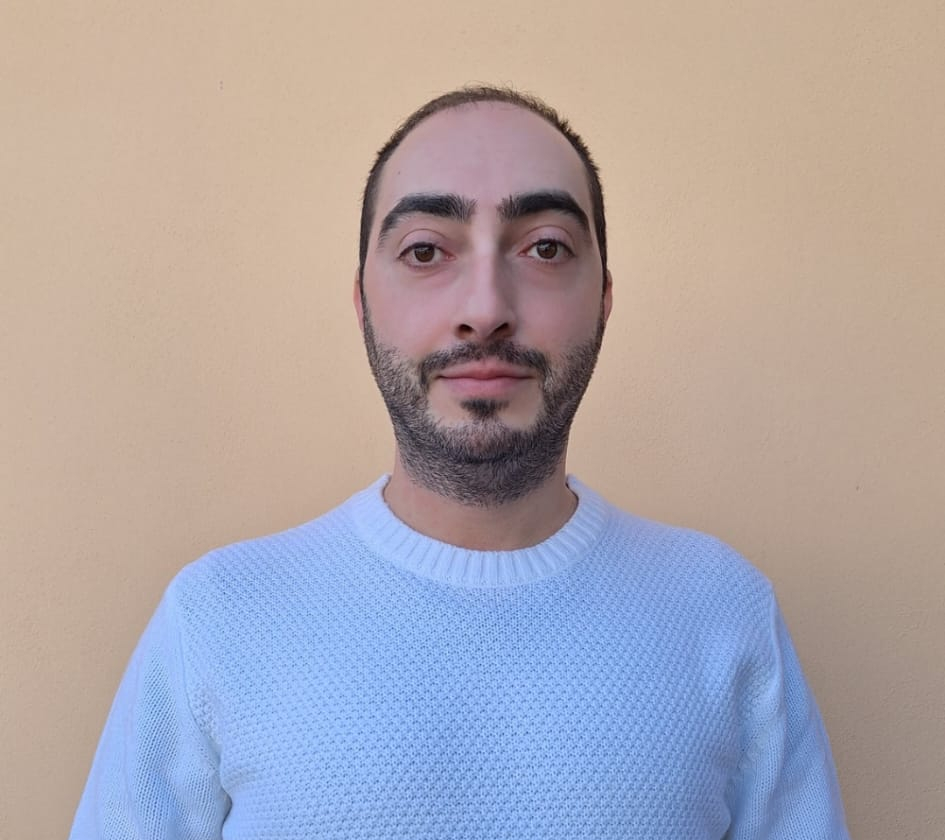
\includegraphics[height=4.2cm]{profile.jpg}};
        \end{tikzpicture}
    \end{center}


% === DATI PERSONALI ===
\end{minipage}%
\hfill
\begin{minipage}[t]{0.70\textwidth}
    \vspace{-0.4cm}
    {\Huge \textbf{\textcolor{mainblue}{Angelo Cassella}}}\\[1pt]
    %\textbf{\textcolor{mainblue}{Ingegnere Informatico | Full Stack Developer | IT Security}}\\
    \textbf{\textcolor{mainblue}{Full Stack Developer | IT Security}}\\
    \rule{\textwidth}{0.4pt}\\[1pt]

    \begin{tabularx}{\textwidth}{@{}l X@{}}
        \faCalendar & \textbf{Data di nascita:} 16/11/1992 \\
        \faChild & \textbf{Luogo di nascita:} Telese Terme (BN), Italia \\
        \faGlobe & \textbf{Nazionalità:} Italiana \\
        \faMars & \textbf{Sesso:} Maschile \\
        \faPhone & \textbf{Telefono:} (+39) 3285633712 \\
        \faEnvelope & \textbf{Email:} \href{mailto:angel.cass92@gmail.com}{angel.cass92@gmail.com} \\
        \faEnvelopeOpenText & \textbf{Pec:} \href{mailto:angel.cass92@pec.it}{angel.cass92@pec.it} \\
        \faSkype & \textbf{Skype:} angel.ca92 \\
        \faLinkedin & \textbf{LinkedIn:} \href{https://www.linkedin.com/in/angelo-cassella-b95754349}{angelo-cassella-b95754349} \\
        \faGithub & \textbf{GitHub:} \href{https://github.com/AngeloCassella}{github.com/AngeloCassella} \\
        \faHome & \textbf{Residenza:} Via Orticelli 38, 82033 Cusano Mutri (BN) \\
    \end{tabularx}
\end{minipage}

\vspace{1mm}
\hrulefill

% === PROFILO PERSONALE (SUMMARY) ===
% Sezione cruciale, resa più specifica e orientata ai risultati/obiettivi
% \section*{\faUser \quad Profilo Professionale}
% Ingegnere informatico con forte propensione allo sviluppo Full Stack e alla sicurezza IT, maturata attraverso esperienze su progetti concreti e multidisciplinari. Ho realizzato applicazioni web con Java EE, Servlet e React, progettato architetture client-server, modellato database relazionali e NoSQL, fino alla gestione avanzata di sistemi di autenticazione OAuth2 con Keycloak. Durante il percorso universitario e lavorativo ho approfondito l'uso di strumenti come Git, Docker, ServiceNow, TFS e SAP, sviluppando un approccio pratico e orientato alla soluzione. Capace di adattarmi rapidamente a nuovi contesti, sono motivato a contribuire in ambienti dinamici e innovativi.

% === PROFILO PERSONALE (SUMMARY) ===
% Sezione cruciale, resa più specifica e orientata ai risultati/obiettivi
\section*{\faUser \quad Profilo Professionale}
Appassionato di sviluppo Full Stack e sicurezza IT, ho maturato solide competenze attraverso progetti universitari e professionali, spaziando dalla realizzazione di applicazioni web con Java EE, Servlet e React, alla progettazione di architetture client-server e database relazionali/NoSQL, fino alla gestione avanzata di sistemi di autenticazione OAuth2 con Keycloak. Ho consolidato la mia preparazione con l’uso di strumenti come Git, Docker, ServiceNow, TFS e SAP, sviluppando un approccio pratico, analitico e orientato alla soluzione. Sono una persona dinamica, curiosa e versatile, in grado di adattarsi rapidamente a nuovi ambienti tecnologici. Sto per conseguire la Laurea in Ingegneria Informatica, coronando un percorso che mi ha già permesso di operare con autonomia e visione tecnica.

\vspace{0mm} % Spazio leggermente aumentato

\hrulefill

% === ESPERIENZA LAVORATIVA ===
\section*{\faBriefcase \quad Esperienza Lavorativa}
\begin{itemize}[leftmargin=*]
  \item \textbf{\textcolor{mainblue}{Service Desk 50 - ENI}}\\
  \textbf {Innovaway s.p.a., Benevento \quad {[17/02/2022 - 31/07/2025]}}\\
  servizio prestato per ENI s.p.a. come service desk 50, orientato alla risoluzione di problemi, incident e ticket svolto a fornire assistenza, supporto tecnico e informativo, con lo scopo dunque di fornire indicazioni o risolvere problemi su utenze, software, hardware e apparecchiature elettroniche, usufruendo di tecnologie e applicativi informatici, utilizzando app del tipo ServiceNow e SAP. aver svolto progetti come MFA Authenticator, firme digitale DIKE e alto.
  
  \item \textbf{\textcolor{mainblue}{Tirocinio formativo - IT Security Specialist}}\\
  \textbf {CST Consorzio Sannio, Benevento \quad {[12/09/2019 – 26/11/2019]}}\\
  Ho svolto attività di gestione di Windows Server, implementando le Misure Minime di Sicurezza e occupandomi della creazione e gestione di VDI (Virtual Desktop Infrastructure basate su Hyper-V). Ho inoltre svolto operazioni di configurazione di backup per sistemi informatici, utilizzo di QGIS per analisi geografiche e sviluppo di script per l'automazione e l'ottimizzazione dei processi IT.

  \item \textbf{\textcolor{mainblue}{Geometra (libera professione e collaborazione)}}\\
  \textbf {Vari studi tecnici, Benevento \quad {[ 05/09/2011 – 30/03/2019]}}\\
  Ho acquisito esperienza come geometra, occupandomi di rilievi, disegno tecnico CAD 2D e 3D, computi metrici, contabilità lavori, gare d’appalto e gestione della sicurezza sul lavoro. Ho collaborato con professionisti e aziende nel settore edile, inclusi impianti elettrici e fotovoltaici, contribuendo a progetti pubblici e privati. Utilizzando software come AutoCAD, Revit la suite di ACCA e altri.
\end{itemize}

\hrulefill

% === ISTRUZIONE E FORMAZIONE ===
\section*{\faGraduationCap \quad Istruzione e Formazione}
\begin{itemize}[leftmargin=*]
  \item \textbf{\textcolor{mainblue}{Laurea Triennale in Ingegneria Informatica}}\\
  \textbf {Università Giustino Fortunato, Benevento \quad {[24/01/2023 - in corso]}}\\
  Città: Benevento | Paese: Italia\\
  Durante il mio percorso in Ingegneria Informatica ho sviluppato progetti stimolanti in ambito Java EE con Servlet, applicazioni client-server, backend web in HTML/JavaScript, modellazione UML e database relazionali e NoSQL. Ho lavorato anche su sistemi embedded con Arduino e, come progetto finale, ho realizzato un sistema di autenticazione avanzato basato su OAuth2 e Keycloak.

  \item \textbf{\textcolor{mainblue}{Corso Full Stack Web Developer}}\\
  \textbf {Musa Formazione, Roma \quad {[15/06/2024 – 17/02/2025]}}\\
  Formazione per impara a Sviluppare Siti Web sia lato front-end che back-end usando: HTML e CSS, Laravel, JavaScript, PHP e MySql, Bootstrap e React., 00198 ROMA (Italia)\\
  Certificazioni: Front End Developer, Back End Developer

  \item \textbf{\textcolor{mainblue}{Tester ISTQB}}\\
  \textbf {Innovaway spa, Benevento \quad {[02/09/2024 – 22/11/2024]}}\\
  Città: Benevento | Paese: Italia\\
  Svolto un corso interno alla società Innovaway riguardante il Tester ISTQB con esperienza nell'utilizzo di ALM per la gestione e il monitoraggio dei test. Specializzato nella User Acceptance Testing (UAT) e nell'utlima fase prima della messa in produzione. svolto e superato anche test interni per la selezione.

  \item \textbf{\textcolor{mainblue}{Java EE Developer}}\\
  \textbf {Udemy (online) \quad {[28/10/2020 – 16/03/2021]}}\\
  Progettazione applicazioni Java Enterprise con servlet e tomcat per scrivere applicazioni web complesse!
  
  \item \textbf{\textcolor{mainblue}{Corso base GDPR}}\\
  \textbf {Dati360.it (online) \quad {[27/03/2020]}}\\
  corso base GDPR regolamento 679/2016

\newpage

  \item \textbf{\textcolor{mainblue}{Corso IFTS Tecnico per la sicurezza delle reti e dei sistemi - IT Security Specialist}}\\
  \textbf {Scuola La Tecnica S.r.l., Benevento \quad {[08/04/2019 – 20/12/2019]}}\\
  Città: Via Falcone e Borsellino n. 1, 82100 - Benevento (BN) | Paese: Italia | Livello NQF: certificati di fine corso \\
  Il corso IFTS è stato strutturato in 800 ore di cui 320 per un percorso formativo e scolastico e 480 di stage presso aziende e società abilitate nel settore specifico. Grazie proprio a questa attività ho potuto comprendere meglio tutto il sistema dell’informatizzazione, vista sotto diversi aspetti. Ho approfondito conoscenze già acquisite, ma soprattutto appreso e imparato cose nuove.
  IFTS, 800 ore (320 teoria + 480 stage).

  \item \textbf{\textcolor{mainblue}{Adobe Photoshop CC}}\\
  \textbf {Udemy (online) \quad {[29/03/2019]}}\\
  Livello NQF: certificato di fine corso n. UC-32MCJXH3

  \item \textbf{\textcolor{mainblue}{EIPASS 7 moduli user}}\\
  \textbf {Scuola La Tecnica, Benevento \quad {[07/09/2018]}}\\
  Città: Via Falcone e Borsellino n.1 82100 | Paese: Italia | Livello NQF: certificato n. QASRUEMSCE
  
  \item \textbf{\textcolor{mainblue}{Diploma di abilitazione all'esercizio all'esercizio della libera professione di geometra}}\\
  \textbf {Galilei-Vetrone, Benevento \quad {[17/12/2015]}}\\
  Città: Benevento (BN) | Paese: Italia | Livello NQF: voto: 63/100

  \item \textbf{\textcolor{mainblue}{Diploma si scuola Superiore}}\\
  \textbf {IIS Carafa Giustiniani, Cerreto Sannita \quad {[06/07/2011]}}\\
  Città: Cerreto Sannita (BN) | Paese: Italia | Livello NQF: voto: 62/100\\
  Geometra Corso Brocca

  \item \textbf{\textcolor{mainblue}{Attestato Corso Chitarra Classica}}\\
  \textbf {Conservatorio Nicola Sala, Benevento \quad {[2005–2011]}}\\
  Città: Benevento (BN) | Paese: Italia\\
  Attestato di frequenza
\end{itemize}

\hrulefill

% === COMPETENZE LINGUISTICHE ===
\section*{\faLanguage \quad Competenze Linguistiche}
\textbf{Italiano:} madrelingua\\
\textbf{Inglese:} livello B1 (lettura, scrittura, ascolto, parlato)

\hrulefill

% === COMPETENZE DIGITALI ===
\section*{\faCode \quad Competenze Digitali}
\begin{multicols}{2}
\textbf{\textcolor{mainblue}{Reti e sistemi}}\\
CISCO (CCNA1, CCNA2, CCENT), Windows Server, Hyper-V, VPN, firewall, backup, QGIS

\textbf{\textcolor{mainblue}{Sviluppo web e software}}\\
HTML, CSS, JavaScript, PHP, Laravel, React, Redux Toolkit, Java EE, Servlet, REST API, Bootstrap, Tomcat

\textbf{\textcolor{mainblue}{Database}}\\
MySQL, Workbench, Access, XAMPP

\textbf{\textcolor{mainblue}{Tools e sistemi}}\\
Git, Docker, Maven, Eclipse, Visual Studio Code, ServiceNow, SAP

\textbf{\textcolor{mainblue}{Sistemi operativi}}\\
Windows, Linux (Ubuntu, Debian), macOS

\textbf{\textcolor{mainblue}{CMS e grafica}}\\
WordPress, Photoshop, Lightroom, Premiere, Final Cut

\textbf{\textcolor{mainblue}{Software tecnici}}\\
AutoCAD, Revit, ACCA, QGIS, laser scanner

\textbf{\textcolor{mainblue}{Altri strumenti}}\\
Office, Google Suite, piattaforme didattiche, dattilografia, Reflex e Drone
\end{multicols}

\hrulefill

% === CERTIFICAZIONI IN DUE COLONNE ===
\section*{\faCertificate \quad Certificazioni}
\begin{multicols}{2}
\begin{itemize}[leftmargin=*]
  \item Front End Web Developer — Musa Formazione
  \item Back End Web Developer — Musa Formazione
  \item Google Analytics - 138722246
  \item ISTQB Certified Tester (in sede) — Innovaway
  \item Java EE Developer — Udemy
  \item GDPR base — Dati360.it
  \item CISCO CCNA1, CCNA2, 
  \item Routing and Switching CCENT
  \item Inglese livello B1 (QCER)
  \item PNL — gestione conflitti lavorativi
  \item Sicurezza lavoratori e videoterminali
  \item EIPASS 7 moduli user — La Tecnica
  \item Adobe Photoshop CC — Udemy
\end{itemize}
\end{multicols}

% === PATENTI E VOLONTARIATO ===
\noindent
\hrulefill
\vspace{0.5em} % piccolo spazio verticale

\begin{minipage}[t]{0.50\textwidth}
    \section*{\faCar \quad \textbf{Patenti}}
    Patente A1\\
    Patente B
\end{minipage}%
\hfill
\begin{minipage}[t]{0.50\textwidth}
    \section*{\faHandsHelping \quad \textbf{Volontariato}}
    \textbf {Protezione Civile Comunale \quad {[dal 15/09/2017]}}\\
    Attività di supporto alla popolazione, prevenzione emergenze\\
    Cusano Mutri (BN)
\end{minipage}

\vspace{0.5em}
\hrulefill

% === DATI PERSONALI ===
\section*{\faUserShield \quad Trattamento dei Dati Personali}
Autorizzo il trattamento dei miei dati personali ai sensi del \href{https://www.garanteprivacy.it/}{D. Lgs. 196/2003} e del \href{https://eur-lex.europa.eu/legal-content/IT/TXT/?uri=CELEX%3A32016R0679}{Regolamento UE 2016/679 (GDPR)}, esclusivamente per finalità di selezione del personale.

\vspace{5mm}
\textit{Cusano Mutri (BN), 16-07-2025}
% \textit{Cusano Mutri (BN), \today}

\end{document}
